\documentclass{article}

\usepackage[utf8]{inputenc}
\usepackage{natbib}
\usepackage{graphicx}
\usepackage{hyperref}
\usepackage{xcolor}
\usepackage[margin=1in]{geometry}

\title{
    Smart Dam \\
    \large Applicazioni e Servizi Web
}

\author{\href{mailto:emalama@studio.unibo.it}{Emanuele Lamagna} - 000725342\\\href{mailto:filippo.barbari@studio.unibo.it}{Filippo Barbari} - 0001052391\\\href{mailto:filippo.benvenuti3@studio.unibo.it}{Filippo Benvenuti} - 0001027545}
\date{\today}

\begin{document}

\maketitle
\section*{Introduzione}\label{sec:intro}
L'idea è di rivisitare un progetto svolto nell'ambito del corso di laurea triennale di Sistemi Embedded e Internet of Things, che consisteva nella simulazione di una diga smart e monitoraggio del livello idrometrico di un fiume. Il sistema era composto da 5 sottosistemi, descritti dall'immagine \ref{fig:dam-scheme}.
\begin{figure}[h!]
	\centering
	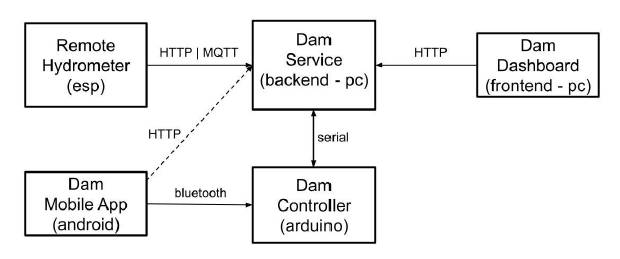
\includegraphics[scale=0.7]{dam-scheme.png}
	\caption{Diagramma dei componenti di DAM}
	\label{fig:dam-scheme}
\end{figure}
L'idea è di rifare da zero backend e frontend utilizzando Node e Vue, oltre all'utilizzo di MongoDB per il salvataggio dei dati. Inoltre per evitare di riesumare Arduino, ESP e l'applicazione mobile (che non concernono il progetto d'esame) simuleremo i sensori/attuatori abilitando tutti i componenti del team allo sviluppo e test del progetto.
Come punto di partenza è stato quindi scelto lo stack MEVN, una versione di MEAN che utilizza come framework Vue invece di Angular. Questa scelta permette l'utilizzo di Javascript anche lato backend (sfruttando Express), dando vita al paradigma "Javascript everywhere" che rende più uniforme e gestibile il codice ed evita molte complicazioni derivanti dall'utilizzo di linguaggi diversi. 
\textcolor{green}{Altro?}

\section{Requisiti}
\textcolor{red}{\textbf{Descrizione delle caratteristiche e funzionalità che il sistema prevede.}} % To remove!
\subsection{Funzionali}
Tenendo in considerazione le anticipazioni al capitolo \nameref{sec:intro} il sistema si riduce a 3 principali componenti:
\begin{enumerate}
	\item \textbf{Dam Backend} (service):
	\begin{itemize}
		\item Salvataggio dati rilevati dai sensori.
		\item Esposizione interfaccia API accessibile tramite HTTP per lettura/salvataggio dati sensori.
	\end{itemize} 
	\item \textbf{Dam Frontend} (Dashboard):
	\begin{itemize}
		\item Grafico real-time relativo all'andamento del livello dell'acqua:
		\begin{itemize}
			\item Linea blu livello corrente acqua.
			\item Linea rossa d'allarme.
			\item Linea gialla d'allerta.
			\item Scelta periodo di aggiornamento grafico.
			\item Possibilità di forzare l'aggiornamento manualmente.
			\item Altri grafici mostranti dati su: temperatura dell'acqua, temperatura esterna, umidità, pressione atmosferica e pioggia.
		\end{itemize}
		\item Panoramic viewer della diga a 360°:
		\begin{itemize}
			\item Zoom in e out, possibilità di entrare in modalità full-screen.
			\item Visione colorata dei livelli di allerta sulla diga.
			\item Ultimo livello rilevato dell'acqua visualizzato sulla diga in tempo reale.
		\end{itemize}
	\end{itemize}
	\item \textbf{Dam Sensor} (Esp, arduino, mobile):
	\begin{itemize}
		\item Simulazione sensori e attuatori IOT:
		\begin{itemize}
			\item Sensore livello dell'acqua.
			\item Sensore del tempo atmosferico.
			\item Attuatore apertura diga.
		\end{itemize}
	\end{itemize}
\end{enumerate}
\subsection{Non funzionali}
Tra i requisiti non funzionali abbiamo catturato le necessità di accessibilità e usabilità del sito, focalizzandoci nello specifico a renderlo usufruibile a soggetti particolari con impedenze sensoriali come:
\begin{itemize}
	\item ablepsia.
	\item ipovisione.
	\item daltonismo.
\end{itemize}

\section{Design}
\textcolor{red}{\textbf{Design dell'architettura del sistema e delle interfacce utente.}}
\textcolor{green}{\textbf{Personas e mockup con BALSAMIQ........ :3}}

\section{Tecnologie}
\textcolor{red}{\textbf{Tecnologie adottate e motivazioni.}}
Di seguito l'elenco delle tecnologie adottate, come le abbiamo usate e perché sono state scelte.
\subsection{Node}
Node.js\cite{node} è un runtime JavaScript costruito sull'engine di Chrome V8. In quanto runtime Javascript asincrono event-driven, Node.js è progettato per costruire applicazioni network scalabili. Node.js è costituito da un event-loop a livello di runtime al contrario di altri sistemi che lo includono come libreria da chiamare con una chiamata bloccante. Il meccanismo ad event-loop potrebbe sembrare CPU intensive, ma in realtà se non c'è lavoro da svolgere Node.js va in sleep rilasciando la maggior parte delle risorse, ma rimanendo pronto a reagire agli eventi nel minor tempo possibile.
\\
\textcolor{green}{Perchè abbiamo usato Node?}

\subsection{Vue}
Vue\cite{vue} è un framework in Javascript per costruire interfacce utente tramite l'uso di HTML, CSS e Javascript. Inoltre fornisce un modello di programmazione dichiarativo e basato sui componenti che aiuta a sviluppare efficientemente le interfacce utente, che siano semplici o complesse. Vue è progettato per essere flessibile e adottabile in modo incrementale, a seconda dei casi d'uso Vue può essere usato in diversi modi:
\begin{itemize}
	\item Potenziare HTML statico senza un passaggio di build.
	\item Incorporarsi come componente Web in qualsiasi pagina.
	\item Applicazioni Single-Page (SPA).
	\item Fullstack / Server-Side-Rendering (SSR).
	\item Jamstack / Static-Site-Generation (SSG).
	\item Può essere mirato allo sviluppo per Desktop, Mobile, WebGL o addirittura per terminale.
\end{itemize}
Nel nostro particolare caso tra Options API e Composition API abbiamo deciso di adottare il primo, Options API, come stile di programmazione, in quanto abbiamo pensato che rispecchiasse meglio l'idea che abbiamo di organizzazione del codice, bisogna inoltre sottolineare che i due stili sono del tutto equivalenti, infatti il primo è internamente costruito basandosi sul secondo, si tratta in tutto e per tutto del famoso "zucchero sintattico" che ci aiuta a mantenere alta la leggibilità del codice.\\
La scelta di usare Vue è stata quasi automatica, una volta aver esplorato la semplicità e le opportunità che mette a disposizione, abbiamo notato che per quello che volevamo realizzare molteplici aspetti del nostro progetto erano già coperti dal framework di Vue, questo ci apriva la strada ad un'implementazione ben organizzata e robusta diventando all'unisono la scelta perfetta per procedere.

\subsection{ApexChart}
ApexCharts\cite{apexcharts} è una moderna libreria di grafici che aiuta gli sviluppatori a creare visualizzazioni eleganti e interattive per pagine web. È un progetto open-source sotto la licenza MIT ed è di uso gratuito per applicazioni commerciali.\\
L'integrazione di grafici con ApexCharts è tanto semplice quanto può esserlo considerando la completezza dei documenti di riferimento (docs) e i 100+ esempi pronti ad essere usati.\\
\begin{figure}[h!]
	\centering
	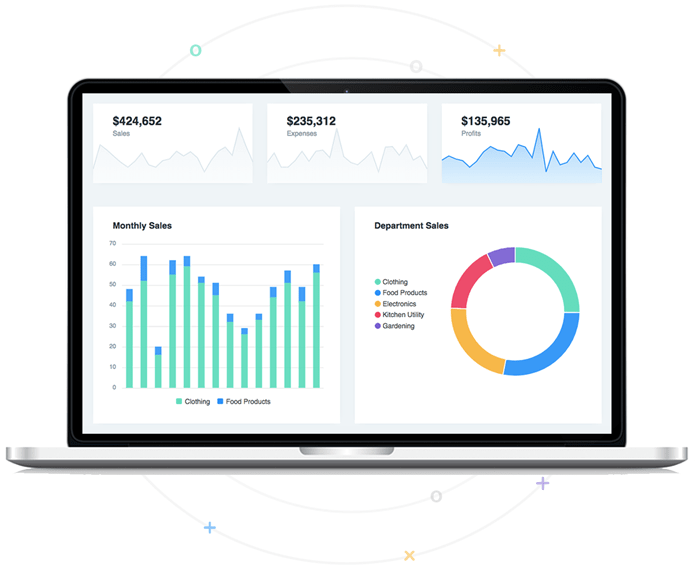
\includegraphics[scale=0.7]{apexchart.png}
	\caption{Piccolo esempio di cosa è possibile fare tramite ApexCharts}
	\label{fig:apexchart}
\end{figure}
Tenendo in considerazione che ApexCharts offre la possibilità di integrarsi tramite Vue, viene automatico pensare che la scelta di questo framework sia ottima, infatti è di facile integrazione all'interno del codice senza sporcarlo con costrutti strani o particolari che andrebbero solamente a danneggiare la leggibilità dei nostri sorgenti, inoltre osservando l'immagine \ref{fig:apexchart} si nota qualche esempio di grafico ottenibile, in questo caso non possiamo apprezzare gli aggiornamenti in tempo reale, ma come si vedrà nel nostro sito, ApexCharts offre grafici in grado di aggiornarsi dinamicamente tramite animazioni fluide ed eleganti.\\
Avendo trovato comodo ed efficiente questo framework, lo abbiamo adottato per la principale visualizzazione di dati dei sensori del nostro progetto.

\subsection{Photo Sphere Viewer}
Photo-Sphere-Viewer\cite{photo-sphere-viewer} è una libreria Javascript usabile per realizzare panorami a 360° tra cui:
\begin{itemize}
	\item \textbf{Spheres and cubemaps}: può visualizzare panorami standard equirettangolari e cubemaps.
	\item \textbf{Touchscreen, gyroscope and VR}: Interazioni semplici e orientate all'utente su tutti i tipi di dispositivo.
	\item \textbf{Markers system}: Visualizza testo, immagini e addirittura aree dinamiche direttamente sull'immagine renderizzata.
	\item \textbf{Fully configurable}: Diverse opzioni, metodi ed eventi consentono un'integrazione profonda nel sito in progettazione.
	\item \textbf{Plugins}: Nuovi plugin aggiungono nuove funzionalità senza sporcare la libreria principale.
	\item \textbf{Videos}: Supporto per i video.
\end{itemize}
La scelta di Photo Sphere Viewer viene naturale considerando i requisiti del nostro progetto, ogni punto di cui abbiamo bisogno è semplicemente implementabile tramite l'uso di una qualche funzionalità già presente all'interno di questa libreria, questo ci consente di concentrarci su aspetti più importanti del nostro sito piuttosto che perdere tempo a reinventare la ruota per realizzare piccole funzionalità.

\subsection{Axios}
Axios\cite{axios} è un client HTTP basato sulle promise per Node.js e il browser, è isomorfo in quanto può girare su Node.js o browser con la stessa codebase. Se nel server-side usa la libreria di Node.js nativa http module, mentre se su client (browser) usa XMLHttpRequests.
Tra le principali funzionalità abbiamo:
\begin{itemize}
	\item Fare richieste XMLHttpRequests da browser.
	\item Fare richieste http da Node.js.
	\item Supporta la API delle promise.
	\item Intercettare richieste e risposte.
	\item Trasformare i dati di richieste e risposte.
	\item Cancellare le richieste.
	\item Trasformazione automatica per i dati JSON.
	\item Supporto lato client alla protezione contro XSRF.
\end{itemize}
La scelta di usare Axios è stata fatta considerando le sue utilità lato client e l'ottima gestione dei dati JSON, semplificandoci ancora una volta il lavoro da fare per gestire le richieste e i dati in esse contenuti. Inoltre Axios si integra perfettamente con Vue, offrendoci ancora una volta un uso pulito e intuitivo, grazie a queste considerazioni non abbiamo avuto dubbi al momento di scegliere quale framework http usare lato client.

\subsection{Express}
Express\cite{express} è un framework web per Node.js che non conosce rivali, in questo ambito è praticamente la scelta migliore considerando la sua efficienza e velocità, bisogna inoltre considerare il suo fascino di minimalità, racchiude infatti tutte le funzionalità di un qualsiasi Web Server, senza aggiungere overhead, risultando quindi in un framework per quanto possibile leggero e funzionale, tra i suoi punti forti notiamo:
\begin{itemize}
	\item \textbf{Web Applications}: Framework minimale e flessibile per applicazioni web che fornisce facilitazioni di sviluppo sia web che per applicazioni mobile.
	\item \textbf{APIs}: Considerando la vastità di utilità HTTP come metodi e middleware a disposizione diventa davvero facile e veloce costruire una robusta API.
	\item \textbf{Performance}: Fornisce un sottile layer di fondamenta per applicazioni web senza oscurare tutte le potenzialità di Node.js.
	\item \textbf{Frameworks}: Molti framework noti e più utilizzati usano express come base di funzionamento.
\end{itemize}
Grazie a queste caratteristiche abbiamo deciso di usare Express per realizzare la parte server del DAM Backend, in questo modo siamo stati in grado di realizzare un'API responsive che ci mettesse a disposizione i dati raccolti dai sensori e che allo stesso modo raccogliesse i dati da questi per memorizzarli \ref{sub:mongo}, abbiamo inoltre testato l'efficienza di Express simulando un carico di lavoro oneroso tramite richieste costruite Ad Hoc, concludendo che per le nostre necessità tale framework fosse più che sufficiente e in grado di sostenere il nostro carico di lavoro.

\subsection{MongoDB}\label{sub:mongo}
MongoDB è un database cross-platform e document oriented che fornisce alte performance, alta disponibilità e facile scalabilità, MongoDB lavora sul concetto di database, collezioni e documenti:
\begin{itemize}
	\item \textbf{Database}: Un container fisico per le collezioni, ogni database possiede il suo personale gruppo di file nel file system, un singolo MongoDB server tipicamente ha più databases.
	\item \textbf{Collection}: Un gruppo di documenti MongoDB, è l'equivalente di una tabella in un RDBMS (Relational DataBase Management System). Le collezioni non forzano l'uso di uno schema, i documenti all'interno di una collezione possono avere diversi campi, comunque tipicamente i documenti all'interno di una stessa collezione hanno scopo similare o comunque sono semanticamente collegati.
	\item \textbf{Document}: Un gruppo di coppie chiave-valore, i documenti hanno schema dinamico rendendo possibile avere gruppi di campi e strutture differenti anche all'interno di una stessa collection.
\end{itemize}
Tra le principali caratteristiche di MongoDB abbiamo:
\begin{itemize}
	\item \textbf{Fast build}: Documenti flessibili e di veloce costruzione con un'interfaccia unificata per le query.
	\item \textbf{Scale further}: Che siano pochi o siano tanti, MongoDB è in grado di soddisfare un qualsiasi numero di richieste (purché ragionevole).
	\item \textbf{Sleep better}: Alta disponibilità, protezione dell'integrità dei dati, sicurezza e adattamento agli standard per il workload più critico.
	\item \textbf{For developers}: Essendo costruito da sviluppatori per metterlo a disposizione di altri sviluppatori, MongoDB diventa intuitivo e di facile utilizzo per chi è abituato a sviluppare.
\end{itemize}
La libertà di utilizzo, la semplicità d'intuito e la flessibilità di quello che si può costruire sono state le principali motivazioni per cui abbiamo scelto di usare MongoDB, inoltre la sua efficienza è un'esperienza che ogni sviluppatore dovrebbe fare.

\subsection{Docker}
Docker rende lo sviluppo efficiente e prevedibile, rimuove le ripetizioni nella configurazione dei tasks e nel ciclo di sviluppo per un'esperienza di velocità e facilità nel portarsi dietro sistemi e applicazioni di sviluppo, sia Desktop che Cloud. Docker offre UIs, CLIs, APIs e sicurezza studiati apposta per lavorare assieme durante tutto il ciclo di vita di consegna del progetto. Tra i principali utilizzi ecco i vantaggi di usare Docker:
\begin{itemize}
	\item \textbf{Build}
	\begin{itemize}
		\item Partire avvantaggiato nel coding usando le immagini di Docker per sviluppare efficientemente le proprie applicazioni sia per Windows che per Mac, creare applicazioni multi-container utilizzando Docker compose.
		\item Integrare con i propri tools preferiti la pipeline di sviluppo, Docker funziona con tutti gli strumenti di sviluppo inclusi VS Code, CircleCI e GitHub.
		\item Impacchettare le applicazioni come immagini contenitori portatili per eseguire in ogni ambiente consistentemente come Kubernetes, AWS ECS, Azure ACI, Google GKE e molto altro.
	\end{itemize}
	\item \textbf{Share}
	\begin{itemize}
		\item Sfruttare i contenuti fidati di Docker, incluse le immagini officiali di Docker e quelle verificare e pubblicate nel Dcoker Hub Repository.
		\item Innovare collaborando con i compagni di team e altri sviluppatori semplicemente pubblicando le immagini su Docker Hub.
		\item Personalizzare l'accesso alle immagini con un control-access basato sui ruoli e ricevere notifiche sulle attività interne con Docker Hub Audit Logs.
	\end{itemize}
	\item \textbf{Run}
	\begin{itemize}
		\item Rilasciare più applicazioni senza alcun problema essendo sicuri che gireranno su ogni ambiente allo stesso modo, includendo il design, il testing, lo staging e la production, che siano desktop o basate sul cloud.
		\item Rilasciare le proprie applicazioni in container separati indipendenti e in diversi linguaggi, riducendo così i rischi di conflitto tra linguaggi, librerie e framework.
		\item Velocizzare lo sviluppo con la semplicità di Docker compose CLI, con un comando lanciare le proprie applicazioni localmente e/o sul cloud con AWS ECS e Azure ACI.
	\end{itemize}
\end{itemize}
Come lo abbiamo usato, perché lo abbiamo usato e quanto sia stato effettivamente comodo usarlo lo rimando alla sezione di \nameref{sec:deploy} dove ne parliamo più specificatamente.

\section{Codice}
In questa sezione andiamo ad analizzare gli aspetti più rilevanti del codice nei vari componenti:
\begin{itemize}
    \item \textbf{Home}: qui sono mostrati i dati più importanti relativi alla diga (l'aggiornamento in tempo reale sarà mostrato nel component Graph).
	\item \textbf{Panorama}: come già accennato abbiamo utilizzato Photo-Sphere Viewer per fornire un'immagine panoramica della diga. Sono stati aggiunti due elementi grafici:
    	\begin{itemize}
    	    \item evidenziamento delle zone della diga relative al livello di allerta
    	    \item icona posizionata al livello corrente dell'acqua, e in constante aggiornamento all'arrivo dei dati
    	\end{itemize}
	Per queste operazioni sono state sfruttate la longitudine e la latitudine, dati forniti dalla libreria.
	\item \textbf{Graph}: per questo component è stata utilizzata la libreria ApexCharts. Sono stati realizzati due grafici (più precisamente di tipo Area):
	\begin{itemize}
	    \item andamento dell'acqua: mostra l'andamento del livello dell'acqua durante il tempo. Sono stati realizzati pulsanti per cambiare la velocità di aggiornamento dei dati e per forzare l'aggiornamento.
	    \item cambiamento del meteo:  questo comprende 6 grafici diversi, relativi a temperatura dell'acqua, temperatura dell'aria, pressione atmosferica, umidità e pioggia. Ogni grafico è selezionabile attraverso un menù a tendina.
	\end{itemize}
	\item \textbf{Controller}: anche in questo component viene utilizzata la libreria ApexCharts, ma il grafico utilizzato è questa volta è un RadialBar. Con quest'ultimo viene mostrata la percentuale di apertura attuale della diga. Oltre ad esso sono presenti dei pulsanti per modificare a mano l'apertura della diga a diverse percentuali.
\end{itemize}
In tutti i component i dati sono ottenuti con delle chiamate (get o post) effettuate grazie ad Axios.

\section{Test}
\textcolor{red}{\textbf{Test effettuati sul codice e test con utenti.}}

Simulazione di utilizzo da parte delle personas, questo probabilmente è da fare dopo aver fatto il design.

\subsection{Test automatici}
\subsubsection{jest e supertest}
Qui parlo degli unit test fatti con jest e supertest.
\subsubsection{Lighthouse}
Qui parlo anche della valutazione di performance e accessibilità effettuata con Lighthouse.
\begin{figure}
	\centering
	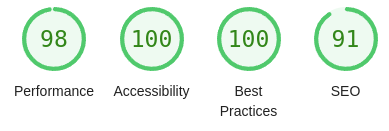
\includegraphics[scale=1]{lighthouse_report_desktop}
	\caption{Report di Lighthouse sulla versione desktop}
	\label{fig:lighthouse_report_desktop}
\end{figure}
\begin{figure}
	\centering
	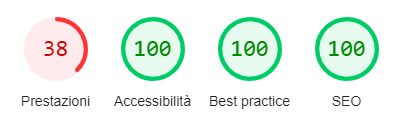
\includegraphics[scale=1]{lighthouse_report_mobile}
	\caption{Report di Lighthouse sulla versione mobile}
	\label{fig:lighthouse_report_mobile}
\end{figure}

\subsection{Exploratory testing}
Qui parlo (forse) dei test manuali effettuati durante lo sviluppo.
\subsection{Test con utenti}
Qui parlo di pecche di usabilità individuate durante lo sviluppo.

\section{Deployment}\label{sec:deploy}
\textcolor{red}{\textbf{Rilascio, installazione e messa in funzione.}}

\textbf{Nella sezione tecnologie l'ultima frase parla di quello che ci si aspetta di trovare qui, inoltre bisogna descrivere dettagliatamente come fare a preparare il progetto e farlo partire perfettamente funzionante.}

\section{Conclusioni}
\textcolor{red}{\textbf{Conclusioni}}
\textcolor{green}{Le relazioni d'esempio sono lunghe un botto mi viene da piangere.}

\bibliographystyle{plain}
\bibliography{references}
\end{document}
